\documentclass[../../main.tex]{subfiles}



\begin{document}
\section{Quicksort and Concurrency}
\subsection{Comparing quicksort implementations}
\subsubsection{Benchmarking environment}
The benchmarks were performed on the following system:

\begin{description}[style=nextline, labelwidth=4.8cm, labelindent=0cm, leftmargin=5cm, font=\normalfont\bfseries]
    \item[Operating System:] Ubuntu 24.04.1 LTS
    \item[RAM:] 32 GB
    \item[CPU:] AMD Ryzen 5 5600G with Radeon Graphics (6 Cores, 2 Threads per Core)
    \item[Compiler:] gcc version 13.2.0
\end{description}


\newpage
\subsubsection{Running time comparison with different numbers of threads}
Here are the results when running the sorting algorithms with varying numbers of threads:

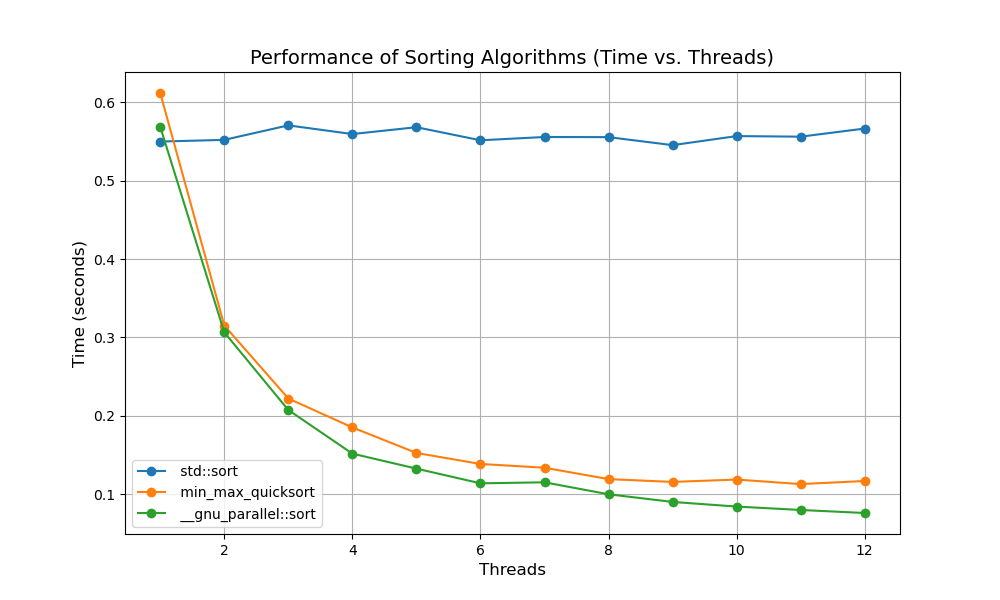
\includegraphics[width=\linewidth]{./running_times.png}

~\\
And here are the performance gains compared to std::sort():

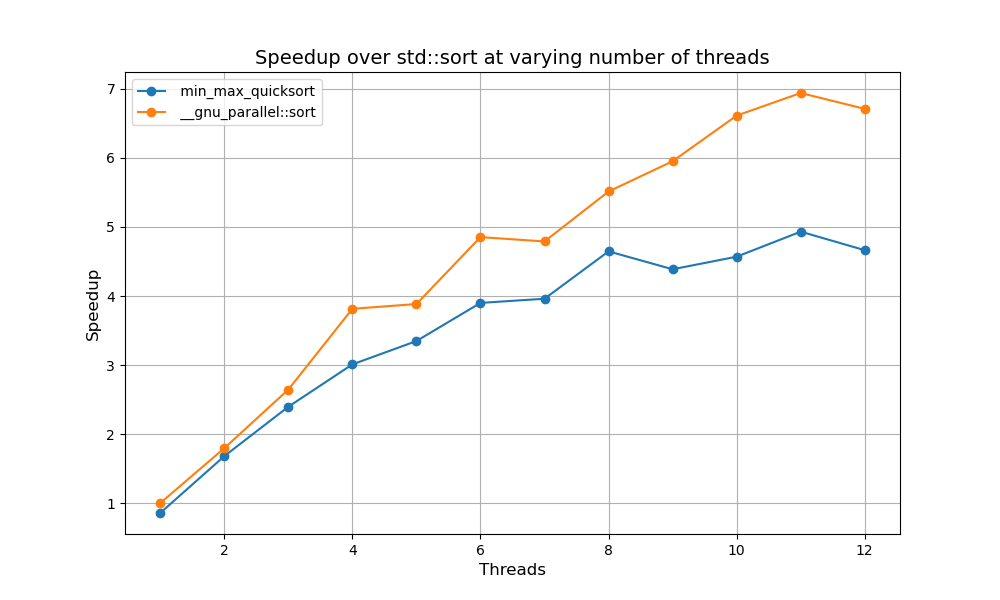
\includegraphics[width=\linewidth]{./speedup.png}


\newpage
\subsubsection{Running time comparison with different array sizes}
Here are the running times with varying array sizes:

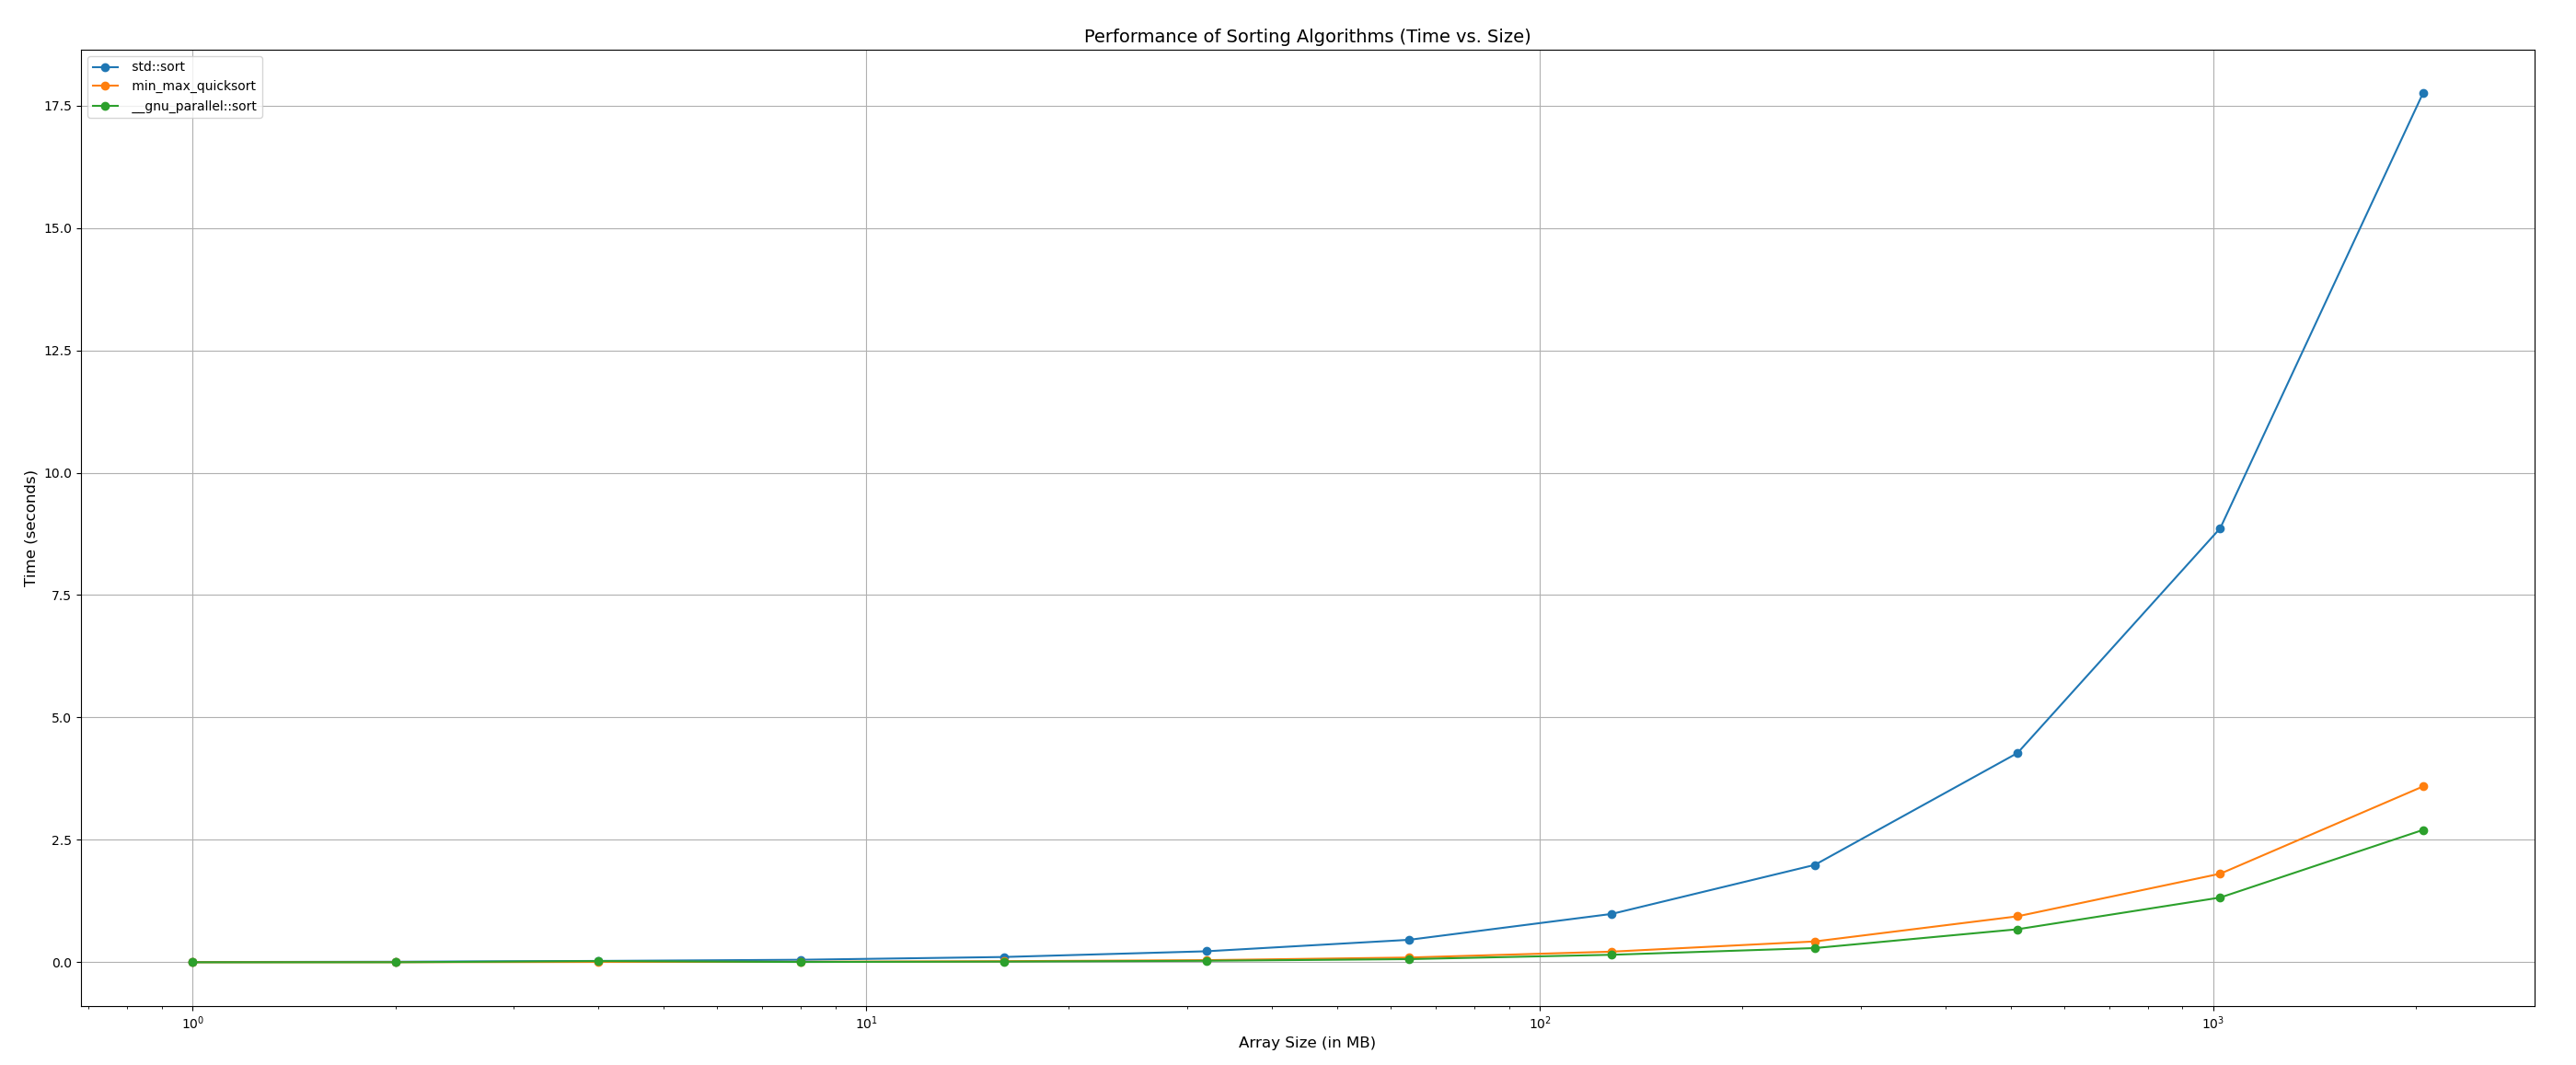
\includegraphics[width=\linewidth]{./running_times_array.png}

~\\
These are the speedups compared to std::sort():

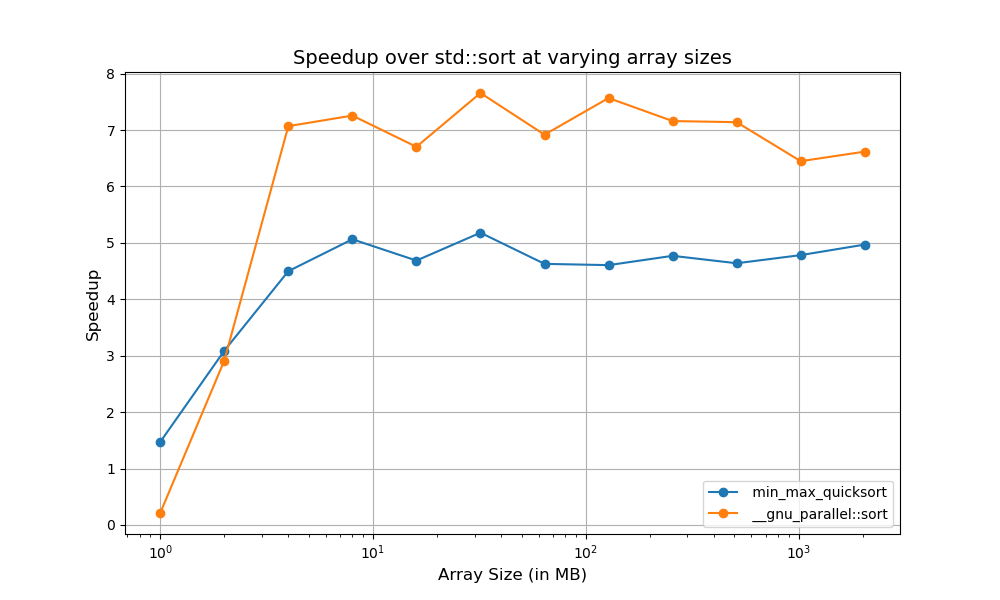
\includegraphics[width=\linewidth]{./speedup_array.png}


~\\
\subsubsection{Explaining the results}
In the first two graphs when measuring the running times and speed ups when varying the threads, we can clearly see that the serial std::sort has a constant running time, whereas both parallel sorting algorithms run quicker with increasing thread number, thus overtaking std::sort already with two threads significantly (almost halving the running time of std::sort).
With further increasing thread number, the running times of the parallel algorithms further decreases.
They are proportional to $\frac{1}{\text{Number of Threads}}$, as one might expect, but the proportionality factor is roughly at 2, meaning there is quite some overhead compared to the optimal running time of $\frac{\text{Serial Running Time}}{\text{Number of Threads}}$.

~\\
Let us now analyze the second two pictures, showing the running times at different array sizes.
The graphs are as expected, the running times of the parallel algorithms is better, even more so for very large array sizes, as in those instances we can fully employ the parallel power of the cpu cores, thus decreasing the running time significantly.
This is why the speedup gets better with increasing array size.
One might think that this speedup is exponential, but it is not (note the logarithmic scale!), it is rather approximately $(\text{Serial Running Time}) \cdot (1 - \frac{1}{12 \cdot E})$, where $E$ is the efficiency $E = \frac{\frac{\text{Serial Running Time}}{\text{Threads}}}{\text{Parallel Running Time}}$, and note that the number of threads on this machine is 12.
Note, that Serial Running Time is expected to grow $\Theta(n \cdot \log(n))$, and so should the speedup.

\end{document}